% fig_schemes.tex -- KV placement schemes tested in the midterm report.
% Build: pdflatex fig_schemes.tex  (standalone; output fig_schemes.pdf)
\documentclass[tikz,border=3pt]{standalone}
\usepackage{helvet}
\renewcommand{\familydefault}{\sfdefault}
\usetikzlibrary{arrows.meta,patterns,positioning,calc,decorations.pathreplacing}

\definecolor{hbm}{HTML}{2a78d6}   % GPU HBM
\definecolor{host}{HTML}{eb6834}  % host (Grace / CPU) pinned memory
\definecolor{slot}{HTML}{1baf7a}  % staging slot
\definecolor{ink}{HTML}{222222}
\definecolor{mute}{HTML}{6b6b6b}

% grid geometry (cm)
\def\W{2.0}    % prefix width
\def\T{0.28}   % tail width
\def\B{0.22}   % drafted-block width
\def\GW{2.5}   % \W+\T+\B
\def\H{1.9}    % grid height (36 layers)

\newcommand{\gridframe}{%
  \foreach \i in {1,...,8} \draw[white,line width=0.5pt] (0,\i*\H/9) -- (\GW,\i*\H/9);
  \draw[ink!45,line width=0.4pt] (\W,0) -- (\W,\H);
  \draw[ink!45,line width=0.4pt] (\W+\T,0) -- (\W+\T,\H);
  \draw[ink,line width=0.5pt] (0,0) rectangle (\GW,\H);
}
\newcommand{\blockhatch}{\fill[pattern=north east lines,pattern color=hbm!80] (\W+\T,0) rectangle (\GW,\H);}
\newcommand{\slots}[1]{% staging slots to the right of the grid; #1 = y of top slot
  \fill[slot!35,draw=slot] (\GW+0.45,#1) rectangle ++(0.55,0.2);
  \fill[slot!35,draw=slot] (\GW+0.45,#1-0.27) rectangle ++(0.55,0.2);
  \node[anchor=north,text=mute,align=center,font=\scriptsize] at (\GW+0.72,#1-0.32) {staging\\$\times 2$ (HBM)};
}

\begin{document}
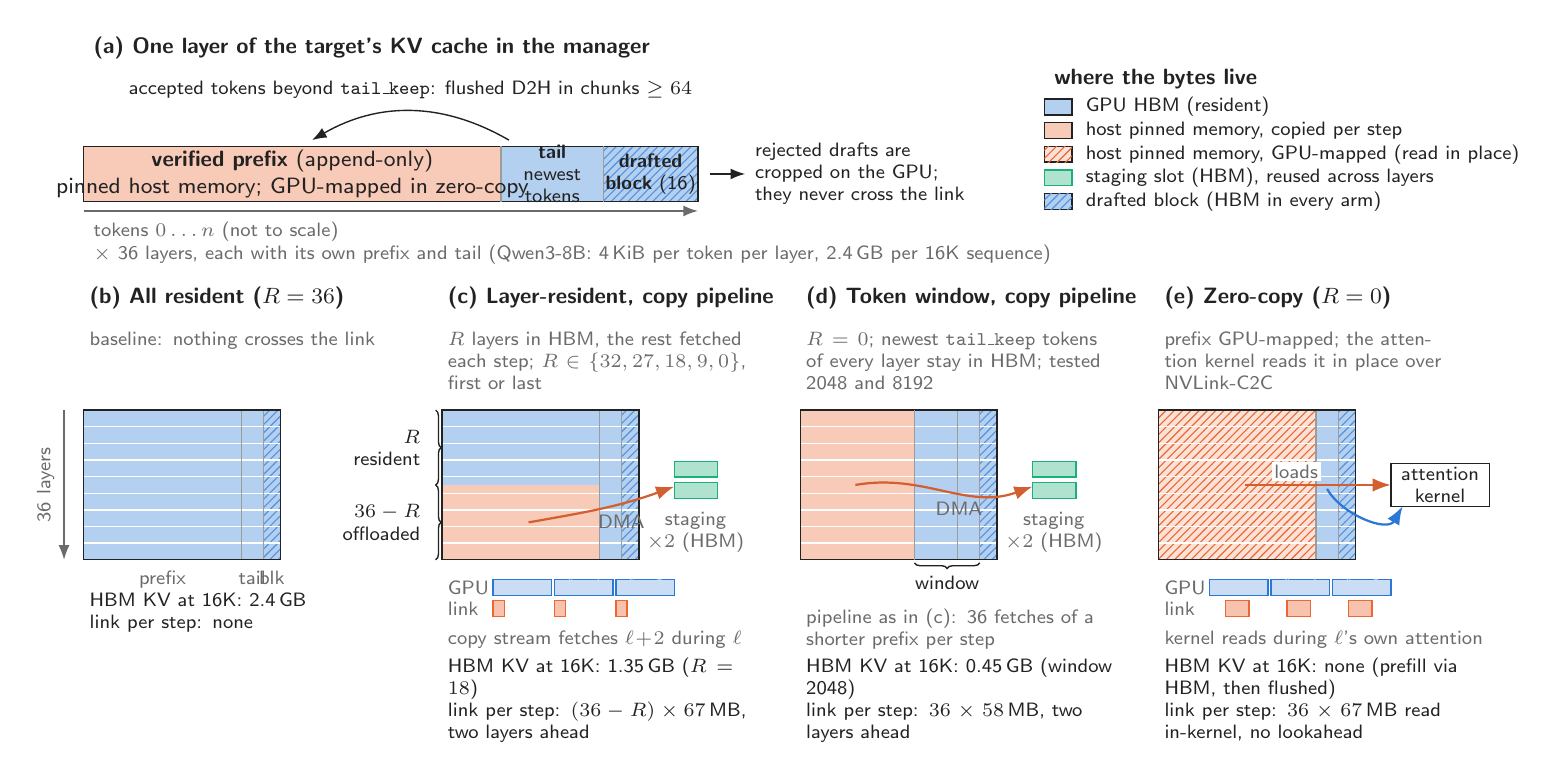
\begin{tikzpicture}[font=\footnotesize,>=Latex,line width=0.5pt,text=ink]

%=================================================================== (a) anatomy
\begin{scope}[shift={(0,4.55)}]
\node[anchor=west,font=\footnotesize\bfseries] at (0,1.95) {(a) One layer of the target's KV cache in the manager};
\def\PW{5.3}\def\TW{1.3}\def\BW{1.2}\def\BH{0.7}
\fill[host!35] (0,0) rectangle (\PW,\BH);
\fill[hbm!35]  (\PW,0) rectangle (\PW+\TW,\BH);
\fill[hbm!35]  (\PW+\TW,0) rectangle (\PW+\TW+\BW,\BH);
\fill[pattern=north east lines,pattern color=hbm!80] (\PW+\TW,0) rectangle (\PW+\TW+\BW,\BH);
\draw[ink] (0,0) rectangle (\PW+\TW+\BW,\BH);
\draw[ink!45] (\PW,0) -- (\PW,\BH); \draw[ink!45] (\PW+\TW,0) -- (\PW+\TW,\BH);
\node[align=center] at (\PW/2,\BH/2) {\textbf{verified prefix} (append-only)\\ pinned host memory; GPU-mapped in zero-copy};
\node[align=center,font=\scriptsize] at (\PW+\TW/2,\BH/2) {\textbf{tail}\\ newest\\ tokens};
\node[align=center,font=\scriptsize] at (\PW+\TW+\BW/2,\BH/2) {\textbf{drafted}\\ \textbf{block} (16)};
% token axis
\draw[->,mute] (0,-0.12) -- (\PW+\TW+\BW,-0.12);
\node[anchor=north west,text=mute,font=\scriptsize] at (0,-0.14) {tokens $0 \ldots n$ (not to scale)};
% annotations
\draw[->,ink] (\PW+0.1,\BH+0.08) to[out=150,in=30] node[above,pos=0.5,font=\scriptsize,align=center,yshift=1pt] {accepted tokens beyond \texttt{tail\_keep}: flushed D2H in chunks $\ge 64$} (\PW-2.4,\BH+0.08);
\draw[->,ink] (\PW+\TW+\BW+0.15,\BH/2) -- ++(0.45,0) node[right,font=\scriptsize,align=left] {rejected drafts are\\ cropped on the GPU;\\ they never cross the link};
\node[anchor=north west,text=mute,font=\scriptsize] at (0,-0.42) {$\times$ 36 layers, each with its own prefix and tail (Qwen3-8B: 4\,KiB per token per layer, 2.4\,GB per 16K sequence)};
\end{scope}

%=================================================================== legend
\begin{scope}[shift={(12.2,4.8)}]
\node[anchor=west,font=\footnotesize\bfseries] at (0,1.3) {where the bytes live};
\fill[hbm!35,draw=ink] (0,0.85) rectangle ++(0.35,0.2); \node[anchor=west,font=\scriptsize] at (0.4,0.95) {GPU HBM (resident)};
\fill[host!35,draw=ink] (0,0.55) rectangle ++(0.35,0.2); \node[anchor=west,font=\scriptsize] at (0.4,0.65) {host pinned memory, copied per step};
\fill[host!20,draw=ink] (0,0.25) rectangle ++(0.35,0.2); \fill[pattern=north east lines,pattern color=host] (0,0.25) rectangle ++(0.35,0.2);
\node[anchor=west,font=\scriptsize] at (0.4,0.35) {host pinned memory, GPU-mapped (read in place)};
\fill[slot!35,draw=slot] (0,-0.05) rectangle ++(0.35,0.2); \node[anchor=west,font=\scriptsize] at (0.4,0.05) {staging slot (HBM), reused across layers};
\fill[hbm!35,draw=ink] (0,-0.35) rectangle ++(0.35,0.2); \fill[pattern=north east lines,pattern color=hbm!80] (0,-0.35) rectangle ++(0.35,0.2);
\node[anchor=west,font=\scriptsize] at (0.4,-0.25) {drafted block (HBM in every arm)};
\end{scope}

%=================================================================== scheme panels
\def\PX{4.55}   % horizontal pitch between panels

% ---------- (b) all resident
\begin{scope}[shift={(0,0)}]
\node[anchor=south west,font=\footnotesize\bfseries] at (-0.05,\H+1.16) {(b) All resident ($R=36$)};
\node[anchor=north west,text=mute,font=\scriptsize,text width=3.9cm,align=left] at (-0.05,\H+1.12) {baseline: nothing crosses the link};
\fill[hbm!35] (0,0) rectangle (\GW,\H);
\blockhatch\gridframe
\draw[->,mute] (-0.25,\H) -- (-0.25,0) node[midway,left,text=mute,font=\scriptsize,rotate=90,anchor=south] {36 layers};
\node[anchor=north,text=mute,font=\scriptsize] at (\W/2,-0.02) {prefix};
\node[anchor=north,text=mute,font=\scriptsize] at (\W+\T/2,-0.02) {tail};
\node[anchor=north,text=mute,font=\scriptsize] at (\W+\T+\B/2,-0.02) {blk};
\node[anchor=north west,align=left,font=\scriptsize,text width=3.9cm] at (-0.05,-0.3) {HBM KV at 16K: 2.4\,GB\\ link per step: none};
\end{scope}

% ---------- (c) layer-resident, copy pipeline
\begin{scope}[shift={(\PX,0)}]
\node[anchor=south west,font=\footnotesize\bfseries] at (-0.05,\H+1.16) {(c) Layer-resident, copy pipeline};
\node[anchor=north west,text=mute,font=\scriptsize,text width=3.9cm,align=left] at (-0.05,\H+1.12) {$R$ layers in HBM, the rest fetched each step; $R\in\{32,27,18,9,0\}$, first or last};
\fill[hbm!35]  (0,\H/2) rectangle (\GW,\H);          % resident first R layers
\fill[host!35] (0,0) rectangle (\W,\H/2);             % offloaded layers: prefix on host
\fill[hbm!35]  (\W,0) rectangle (\GW,\H/2);           % their tail + block in HBM
\blockhatch\gridframe
\draw[decorate,decoration={brace,amplitude=2pt},ink] (-0.08,\H) -- (-0.08,\H/2) node[midway,left=2pt,font=\scriptsize,align=right] {$R$\\ resident};
\draw[decorate,decoration={brace,amplitude=2pt},ink] (-0.08,\H/2) -- (-0.08,0) node[midway,left=2pt,font=\scriptsize,align=right] {$36-R$\\ offloaded};
\slots{\H/2+0.1}
\draw[->,host!90!black,thick] (\W*0.55,\H*0.25) to[out=10,in=200] node[below,pos=0.6,font=\scriptsize,text=mute,xshift=2pt] {DMA} (\GW+0.45,\H/2-0.02);
% mini timeline
\node[anchor=west,text=mute,font=\scriptsize] at (-0.05,-0.35) {GPU};
\node[anchor=west,text=mute,font=\scriptsize] at (-0.05,-0.62) {link};
\foreach \k/\l in {0/$\ell$,1/$\ell\!+\!1$,2/$\ell\!+\!2$} {
  \fill[hbm!25,draw=hbm] (0.65+\k*0.78,-0.45) rectangle ++(0.74,0.2) node[midway,font=\scriptsize] {\l};
  \fill[host!40,draw=host] (0.65+\k*0.78,-0.72) rectangle ++(0.14,0.2);
}
\node[anchor=north west,font=\scriptsize,text=mute] at (-0.05,-0.78) {copy stream fetches $\ell\!+\!2$ during $\ell$};
\node[anchor=north west,align=left,font=\scriptsize,text width=3.9cm] at (-0.05,-1.12) {HBM KV at 16K: 1.35\,GB ($R=18$)\\ link per step: $(36-R)\times 67$\,MB, two layers ahead};
\end{scope}

% ---------- (d) token window, copy pipeline
\begin{scope}[shift={(2*\PX,0)}]
\node[anchor=south west,font=\footnotesize\bfseries] at (-0.05,\H+1.16) {(d) Token window, copy pipeline};
\node[anchor=north west,text=mute,font=\scriptsize,text width=3.9cm,align=left] at (-0.05,\H+1.12) {$R=0$; newest \texttt{tail\_keep} tokens of every layer stay in HBM; tested 2048 and 8192};
\fill[host!35] (0,0) rectangle (\W-0.55,\H);
\fill[hbm!35]  (\W-0.55,0) rectangle (\GW,\H);
\blockhatch\gridframe
\draw[ink!45,line width=0.4pt] (\W-0.55,0) -- (\W-0.55,\H);
\draw[decorate,decoration={brace,amplitude=2pt,mirror},ink] (\W-0.55,-0.04) -- (\W+\T,-0.04) node[midway,below=1pt,font=\scriptsize] {window};
\slots{\H/2+0.1}
\draw[->,host!90!black,thick] (\W*0.35,\H*0.5) to[out=10,in=200] node[below,pos=0.55,font=\scriptsize,text=mute,xshift=2pt] {DMA} (\GW+0.45,\H/2-0.02);
\node[anchor=north west,text=mute,font=\scriptsize,text width=3.9cm,align=left] at (-0.05,-0.5) {pipeline as in (c): 36 fetches of a shorter prefix per step};
\node[anchor=north west,align=left,font=\scriptsize,text width=3.9cm] at (-0.05,-1.12) {HBM KV at 16K: 0.45\,GB (window 2048)\\ link per step: $36\times 58$\,MB, two layers ahead};
\end{scope}

% ---------- (e) zero-copy
\begin{scope}[shift={(3*\PX,0)}]
\node[anchor=south west,font=\footnotesize\bfseries] at (-0.05,\H+1.16) {(e) Zero-copy ($R=0$)};
\node[anchor=north west,text=mute,font=\scriptsize,text width=3.9cm,align=left] at (-0.05,\H+1.12) {prefix GPU-mapped; the attention kernel reads it in place over NVLink-C2C};
\fill[host!20] (0,0) rectangle (\W,\H);
\fill[pattern=north east lines,pattern color=host] (0,0) rectangle (\W,\H);
\fill[hbm!35]  (\W,0) rectangle (\GW,\H);
\blockhatch\gridframe
% attention kernel box
\draw[ink,fill=white] (\GW+0.45,\H/2-0.27) rectangle ++(1.25,0.54) node[midway,align=center,font=\scriptsize] {attention\\ kernel};
\draw[->,host!90!black,thick] (\W*0.55,\H*0.5) -- (\GW+0.45,\H/2) node[pos=0.35,above,font=\scriptsize,text=mute,fill=white,inner sep=1pt,yshift=1pt] {loads};
\draw[->,hbm,thick] (\W+\T/2,\H*0.5-0.05) to[out=-60,in=240] (\GW+0.6,\H/2-0.27);
% mini timeline
\node[anchor=west,text=mute,font=\scriptsize] at (-0.05,-0.35) {GPU};
\node[anchor=west,text=mute,font=\scriptsize] at (-0.05,-0.62) {link};
\foreach \k/\l in {0/$\ell$,1/$\ell\!+\!1$,2/$\ell\!+\!2$} {
  \fill[hbm!25,draw=hbm] (0.65+\k*0.78,-0.45) rectangle ++(0.74,0.2) node[midway,font=\scriptsize] {\l};
  \fill[host!40,draw=host] (0.65+\k*0.78+0.2,-0.72) rectangle ++(0.3,0.2);
}
\node[anchor=north west,font=\scriptsize,text=mute] at (-0.05,-0.78) {kernel reads during $\ell$'s own attention};
\node[anchor=north west,align=left,font=\scriptsize,text width=3.9cm] at (-0.05,-1.12) {HBM KV at 16K: none (prefill via HBM, then flushed)\\ link per step: $36\times 67$\,MB read in-kernel, no lookahead};
\end{scope}

\end{tikzpicture}
\end{document}
